\documentclass[border=10pt]{standalone}
\usepackage{pgfplots}
\pgfplotsset{compat=1.18}
\begin{document}
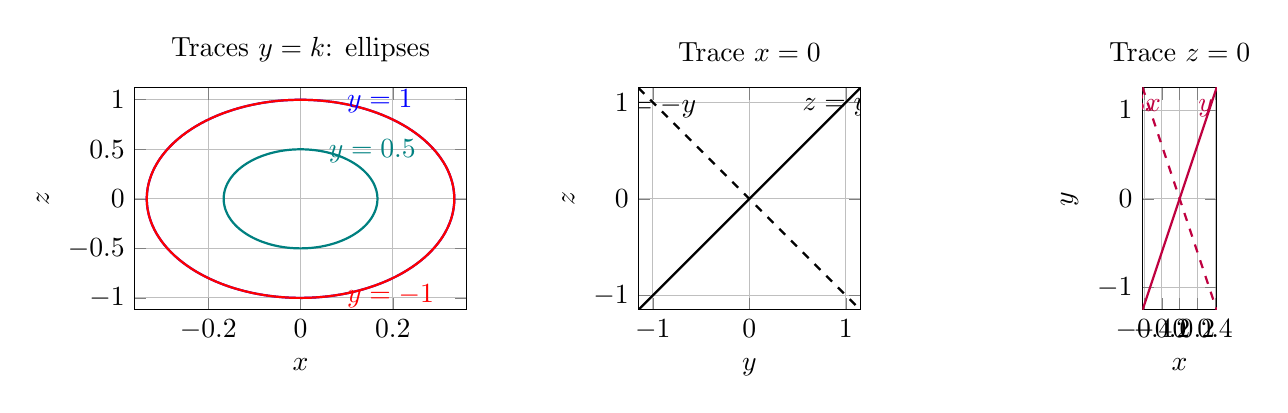
\begin{tikzpicture}
\begin{axis}[
    width=5.8cm, height=4.4cm,
    xlabel={$x$}, ylabel={$z$},
    xmin=-0.36, xmax=0.36, ymin=-1.12, ymax=1.12,
    grid=major,
    title={Traces $y=k$: ellipses}
]
\addplot[domain=0:360, samples=150, thick, blue, no markers] ({cos(x)/3}, {sin(x)});
\addplot[domain=0:360, samples=150, thick, teal, no markers] ({0.5*cos(x)/3}, {0.5*sin(x)});
\addplot[domain=0:360, samples=150, thick, red, no markers] ({cos(x)/3}, {-sin(x)});
\node[blue, anchor=west] at (axis cs:0.08,0.98) {$y=1$};
\node[teal, anchor=west] at (axis cs:0.04,0.48) {$y=0.5$};
\node[red, anchor=west] at (axis cs:0.08,-0.98) {$y=-1$};
\end{axis}

\begin{axis}[
    width=5.8cm, height=4.4cm,
    at={(6.4cm,0)},
    xlabel={$y$}, ylabel={$z$},
    xmin=-1.15, xmax=1.15, ymin=-1.15, ymax=1.15,
    grid=major, axis equal image,
    title={Trace $x=0$}
]
\addplot[domain=-1.15:1.15, samples=50, thick, black, no markers] (x, x);
\addplot[domain=-1.15:1.15, samples=50, thick, black, dashed, no markers] (x, -x);
\node[black, anchor=west] at (axis cs:0.45,0.95) {$z=y$};
\node[black, anchor=east] at (axis cs:-0.45,0.95) {$z=-y$};
\end{axis}

\begin{axis}[
    width=5.8cm, height=4.4cm,
    at={(12.8cm,0)},
    xlabel={$x$}, ylabel={$y$},
    xmin=-0.42, xmax=0.42, ymin=-1.25, ymax=1.25,
    grid=major, axis equal image,
    title={Trace $z=0$}
]
\addplot[domain=-0.42:0.42, samples=50, thick, purple, no markers] (x, 3*x);
\addplot[domain=-0.42:0.42, samples=50, thick, purple, dashed, no markers] (x, -3*x);
\node[purple, anchor=west] at (axis cs:0.10,1.05) {$y=3x$};
\node[purple, anchor=east] at (axis cs:-0.10,1.05) {$y=-3x$};
\end{axis}
\end{tikzpicture}
\end{document}